\newif\ifshowsolutions
\showsolutionstrue
\documentclass{article}
\usepackage{listings}
\usepackage{amsmath}
%\usepackage{subfigure}
\usepackage{subfig}
\usepackage{amsthm}
\usepackage{amsmath}
\usepackage{amssymb}
\usepackage{graphicx}
\usepackage{mdwlist}
\usepackage[colorlinks=true]{hyperref}
\usepackage{geometry}
\usepackage{titlesec}
\geometry{margin=1in}
\geometry{headheight=2in}
\geometry{top=2in}
\usepackage{palatino}
\usepackage{mathrsfs}
\usepackage{fancyhdr}
\usepackage{paralist}
\usepackage{todonotes}
\setlength{\marginparwidth}{2.15cm}
\usepackage{tikz}
\usetikzlibrary{positioning,shapes,backgrounds}
\usepackage{float} % Place figures where you ACTUALLY want it
\usepackage{comment} % a hack to toggle sections
\usepackage{ifthen}
\usepackage{mdframed}
\usepackage{verbatim}
\usepackage[strings]{underscore}
\usepackage{listings}
\usepackage{bbm}
\rhead{}
\lhead{}

\renewcommand{\baselinestretch}{1.15}

% Shortcuts for commonly used operators
\newcommand{\E}{\mathbb{E}}
\newcommand{\Var}{\operatorname{Var}}
\newcommand{\Cov}{\operatorname{Cov}}
\newcommand{\Bias}{\operatorname{Bias}}
\DeclareMathOperator{\argmin}{arg\,min}
\DeclareMathOperator{\argmax}{arg\,max}

% do not number subsection and below
\setcounter{secnumdepth}{1}

% custom format subsection
\titleformat*{\subsection}{\large\bfseries}

% set up the \question shortcut
\newcounter{question}[section]
\newenvironment{question}[1][]
  {\refstepcounter{question}\par\addvspace{1em}\textbf{Question~\Alph{question}\!
    \ifthenelse{\equal{#1}{}}{}{ [#1 points]}: }}
    {\par\vspace{\baselineskip}}

\newcounter{subquestion}[question]
\newenvironment{subquestion}[1][]
  {\refstepcounter{subquestion}\par\medskip\textbf{\roman{subquestion}.\!
    \ifthenelse{\equal{#1}{}}{}{ [#1 points]:}} }
  {\par\addvspace{\baselineskip}}

\titlespacing\section{0pt}{12pt plus 2pt minus 2pt}{0pt plus 2pt minus 2pt}
\titlespacing\subsection{0pt}{12pt plus 4pt minus 2pt}{0pt plus 2pt minus 2pt}
\titlespacing\subsubsection{0pt}{12pt plus 4pt minus 2pt}{0pt plus 2pt minus 2pt}


\newenvironment{hint}[1][]
  {\begin{em}\textbf{Hint: }}{\end{em}}

\ifshowsolutions
  \newenvironment{solution}[1][]
    {\par\medskip \begin{mdframed}\textbf{Solution~\Alph{question}#1:} \begin{em}}
    {\end{em}\medskip\end{mdframed}\medskip}
  \newenvironment{subsolution}[1][]
    {\par\medskip \begin{mdframed}\textbf{Solution~\Alph{question}#1.\roman{subquestion}:} \begin{em}}
    {\end{em}\medskip\end{mdframed}\medskip}
\else
  \excludecomment{solution}
  \excludecomment{subsolution}
\fi

\newcommand{\boldline}[1]{\underline{\textbf{#1}}}

\chead{%
  {\vbox{%
      \vspace{2mm}
      \large
      Machine Learning \& Data Mining \hfill
      Caltech CS/CNS/EE 155 \hfill \\[1pt]
      Miniproject 1\hfill
      Released February $17^{th}$, 2017 \\
    }
  }
}

\usepackage{amsfonts} %Mathbb Fonts
\usepackage{amsmath} %Text in Math
\usepackage{longtable} %Make multi-page tables
\usepackage{enumitem}
\usepackage{graphicx} % Import pics \includegraphics[scale=0.7]{SGD}
\graphicspath{{figures/}} % Change pic path
\usepackage{makecell}
\usepackage[margin=2.25cm]{caption}

\begin{document}
\pagestyle{fancy}

\section{Introduction}
\medskip
\begin{itemize}

    \item \boldline{Group members} \\
    Vaibhav Anand \\
    Nikhil Gupta \\
    Michael Hashe
    
    \item \boldline{Team name} \\
    The Breakfast Club

    \item \boldline{GitHub link} \\
    \href{https://github.com/nkgupta1/CS155-Project2-Poetry-Generation}{https://github.com/nkgupta1/CS155-Project2-Poetry-Generation}
    
    \item \boldline{Division of labour} \\
    Vaibhav Anand: Supervised HMM, Rhyming, Syllables, Report \\
    Nikhil Gupta: Unsupervised HMM, RNN, Report \\
    Michael Hashe: Data Visualization, Report

\end{itemize}

\section{Tokenizing}
\medskip

\subsection{What methods did you use and try to tokenize the sonnets?}
In the supervised HMM models, the y-states were defined by the part of speech (POS) of a word mapped to a unique integer, and the x-observations were represented by each distinct word in the text mapped to a distinct integer. For these models, we used the Natural Language Toolkit (NLTK) library for python to tokenize the sonnets. It allowed us to split each line in the sonnet texts into words and tag them by their part of speech. A total of 34 and 31 distinct part of speech tags were found for the Shakespeare and Spenser texts, respectively. Among these tags, for example, three most popular POS tags were 6039 instances of nouns, 3126 instance of conjunctions, and 2681 instances of adjectives.\\
\indent In the supervised HMM models, we removed the punctuation and possessive apostrophes including: [, : . ; ! ? ) ' ( `s] in pre-processing. This was done to simplify our model with less number of states and by removing nonsensical endings of phrases or sentences in our emissions.
\subsection{Did you have to make changes to the way you tokenized after running the algorithm and seeing the results?}
Initially, we included punctuation as distinct observations in our model, but our model did not appear to train well on them and they broke many lines in a nonsensical manner, so they were removed. We also tried tokenizing the words  by their iambic pentameter and stress as well as giving a unique state for the last word in a line. Although we chose not to do this, the idea was to have distinct(POS) $\times$ distinct(Iambic) $\times$ distinct(part of line) states such that there would be a unique state for every combination of the three concepts. This was partly rejected because there was a better method for terminating a line with a fixed number of syllables, described in Additional Goals, and it would over-complicate the model.

\section{Algorithm}
\medskip
\subsection{What packages did you use for the algorithm?}
We used the supervised and unsupervised HMM code from homework 5 as the base for our HMM models in this project. The NumPy package helped with data manipulation. As mentioned earlier, the NLTK library was useful in tokenizing and labeling parts of speech. For visualization, we used MathPlotLib, GraphViz, NLTK, and NumPy. \\
\indent For the recurrent neural network, we used Keras with a Tensorflow backend to create a sequential model with long short-term memory (LSTM), a type of RNN, layers.
\subsection{What decisions did you have to make when running the algorithm and what did you try? e.g number of states}
We tried various number of states for the unsupervised model. We found that with too few states, the model just kept on generating sequences of nouns. As we kept on increasing the number of states, it was difficult to tell the difference in performance. However, as the number of states increased, so did training time. \\
\indent For the supervised model with rhyming, we tried various levels of rhyming strengths and tolerance, where the rhyming strength denotes the strictness with which a pair of words were considered to rhyme and rhyming tolerance denotes the relative decrease in likelihood if a word did not rhyme when it was supposed to. We found that the lowest rhyming strength possible and low rhyming tolerance of 0.01 was most effective in generating rhymes when training the supervised HMM. \\
\indent Another decision we had to make was how to break up the input and pass it into the model. We tried treating a line as a sequence, a sonnet as a sequence, and all the sonnets as a sequence. We also had to decide whether to keep capitalization and punctuation, both of which we ultimately removed. 
\subsection{How did this affect the sonnets that were generated?}
We found that with too few states, the model was not able to distinguish between the different parts of speech and as such, learned little to no grammar, making poems that made no sense. When treating all the sonnets as a single sequence, we found that the generated poems made less sense than the other methods. Capitalization and punctuation needlessly increased the number of observations for the models so we removed both of these.

\section{Poetry Generation}
\medskip

\subsection{How did you generate your poem?}
The poems from by the supervised and unsupervised HMM models were generated word by word. In particular, we broke up each line into its component words, after stripping them of any punctuation and capitalization. At this point, we fed this set of inputs into the unsupervised HMM and let it train on it. For the RNN, the input was parsed character by character, with punctuation and line breaks kept in, with all capitalization removed. Here is an example of a poem that was generated with an unsupervised model with 30 states trained for 75 iterations: \\
\begin{small}
\texttt{
My before minutes do doth could my stain and that, \\
All thou my of to fee a them gives restore, \\
Basest think thine oerpressed vassal wherewith thy home on thine, \\
Fair in will fire from thy pain more nothing greet, \\
Monument truetelling that clean thee idol tires decay doth away, \\
Fortune threw thee bring self knowst hide that age steal, \\
Self truth forgot first of buds once that favour thy, \\
Alas whilst his needing a teachest doth sleep gored or, \\
Keeps that me sadly i not thee special kept should, \\
Part my than mounted thee will so our these slander, \\
Have you beauty on i my breast praise rich of, \\
And most me waves than prisoner taken of one of, \\
All thee infection now to all remote thy that by, \\
Like his thou away title in my self be of. \\
}
\end{small}
This poem has some semblance of grammar but other than that, is terrible. It has no rhyme, rhythm, or syllable count. It makes no sense. It does not retain Shakespeare's voice. We suspect that the reason it is able to learn some grammar is because individual states are becoming associated with parts of speech. This point is elaborated on in the data visualization section.


\subsection{How did you get your poem to look as much like a sonnet as possible?}
For HMM, we initially created a model that split each line after the last word caused the line to exceed a fixed number of characters such as 60. We later developed a model to split each line by exactly 10 syllables by forcing the last word in the line to complete the 10th syllable. See Additional Goals for our implementation of Shakespearean rhyming and further information about fixed syllable count in the supervised HMM model.
\subsection{What makes sense/what doesn't about the sonnets generated?}
In comparison to the supervised models, we noticed that the sonnets generated by the unsupervised models had more trouble learning grammar and part of speech. This makes sense because the supervised HMM has more information off of which to train. For the unsupervised HMM, it was more common to see words of the same part of speech following each other, when the number of states was not ideal. In particular, the unsupervised model appeared to learn the grammar best when given a medium number of about 10 states, which likely corresponded with the realistic number of important and distinct parts of speech in the text. In the end, we decided to include an emission from the supervised model and not unsupervised in our submission, since it had the advantage of being given POS to learn the grammar better.

\section{Visualization and Interpretation}
For visualization purposes, three models (one each with 5, 10, and 15 hidden states) were trained. We analyzed the top words associated with each model, as well as the frequency with which each state emitted each part of speech, words with certain number of syllables, and the transition frequencies between states.

\medskip

% \subsection{For at least 5 hidden states give a list of the top 10 words that associate with this hidden state and state any common features these groups.}
\subsection{Top Words Associated with each state}
For a list of the most common words associated with each state, please see Appendix A.\\

For the simplest model (5 hidden states), all words are one syllable. Many are repeated between lists, and in particular there appears to be little specialization between states. For the larger model, several two syllable words are represented and words are repeated at a lower frequency. Specifically, each word is repeated an average of 1.389 times in the 5 state model, 1.639 (< 2 * 1.389) times in the 10 state model, and 1.705 (< 3 * 1.389) times in the 15 state model. Clearly, the more advanced model allows for better specialization of each state.

% \subsection{What are some properties of the different hidden states?}
% \subsection{e.g. Correlation between hidden states and syllable counts, connotations of words, etc.}
% \subsection{Make a visual representation of the correlation between states and words}
\subsection{Interpretation of Hidden States}
We consider the possibilities that hidden states learn parts of speech or syllable counts. Our model did not appear to demonstrate iambic pentameter, so we discount the possibility that it learned meter sufficiently well. Graphs are included in Appendices B-E.\\

We first examine how well the models perform at identifying parts of speech. Graphs are included in Appendix B.

We find that the models learn parts of speech quite well. In particular, there is significant specialization amongst states; this trend appears to increase as the number of states rises. As an extreme example, we note that prepositions are only emitted in appreciable quantities in three of the 15 states of our final model. Similar `peaks' are observed for adjectives and pronouns. Nouns are well represented for almost all states in our three models, as should be expected. It is interesting to note that while nouns and conjunctions are both highly represented in the 5 state model (and in the underlying data), they demonstrate disparate behavior for the more complicated models; nouns (at least superficially) are represented more evenly than conjunctions. This differing treatment for differing parts of speech implies that our model is capable of learning grammatical subleties.\\

We next examine how well the models perform at identifying syllable counts. Graphs are included in Appendix C.

We find that the model does not learn to classify words on syllable length very well. In particular, emission rates are nearly identical across the states in the 5 state model. Variations exist for the more complicated models, although they are still fairly insignificant and are likely a side effect of the model learning other factors (namely, parts of speech).\\

We next examine the transition frequencies between different states. These transitions do not explicitly give us information about the meaning of the hidden states, and are presented without further analysis in Appendix D.\\

Finally, we visualize the models as networks. Having concluded that the model most successfully learns parts of speech, we classify nodes by their most ``over-represented'' parts of speech. Specifically, we label nodes by either a.) all parts of speech that it emits at at least half a standard deviation above the mean, or b.) if it emits no part of speech at this frequency, the part of speech that it emits at the highest rate above the mean (measured as the ratio emission frequency / mean). These nodes are connected by directed edges added along high probability state transitions. In particular, a directed edge is added if the transition rate is above the mean; given that most pairs have near 0 probability of transitions, this produces a reasonable number of edges. The graphs are shown in Appendix E.
In analyzing these graphs, it appears that transitions follow (in most cases) `logical' structure; nouns to verbs, adverbs to verbs, adjectives to nouns, etc. The correlation is not perfect, of course; there are an unusually high number of noun to noun transitions, whereas this pattern is actually quite rare. This is likely a result of generally high emission rates for nouns (i.e., it is hard to transition to a state with low noun emission states), and of misclassification of words. In particular, words such as doth and thy are classified as nouns, while they can be used in other contexts.\\

In conclusion, our HMM has learned patterns in Shakespeare's texts primarily through learning transitions between words, and in particular has developed a rudimentary sense of grammar. We note that this is in part a consequence of how our model was trained; if we had trained syllable by syllable instead, the model would likely have focused on other patterns.\\

\section{Additional Goals}
\medskip
We were able to add rhyming and a fixed number of syllables per line to our supervised HMM model. This was done as follows. We acquired packages online that allowed us to check whether two words rhymed and the number of syllables in a word. Using these, we created a rhyming matrix (call this $R$) with dimensions distinct(observations) $\times$ distinct(observations) and filled it with boolean values to represent if a pair of words rhymed. For example, if a row-word and column-word rhymed, it had the value 1 in the matrix 0.01 if not given a ``tolerance" value of 0.01. We also created a one-dimensional vector (call this $S$), which contained the number of syllables for each distinct observation.\\
\indent To implement rhyming and syllable counting, we did not alter the supervised training phase but the emission phase. Once the states were chosen from the HMM using weighted probabilities, we modified the probabilities by which the observations were chosen from them. Let $w$ be the vector of observation probabilities found for a particular state in the observation $O$ matrix. For every line generated in the sonnet, while the number of syllables remaining $l$ in the line was less than 10, we multiplied $w$ for the next word by the syllables vector where values greater than $l$ were thresholded to zero and else were one. This assured that we never created a line over 10 syllables in length. For lines in which the last word needed to rhyme with a previous line by the Shakespearean rhyming scheme, we then multiplied the indices of $w$ that equaled $l$ in the syllables vector by the row of the observation in $R$. Therefore, a word that didn't rhyme would only have a greater probability of being chosen relative to a rhyming word if it originally had greater than 100 times the probability to begin with if $R$ had a tolerance value of 0.01. Therefore, we did not force the last word to rhyme, but increased its weighted probability of becoming chosen.


\section{Extra Credit}
\medskip

\subsection{What did you use to collect more data and what packages did you use for RNN/LSTM?}
We used both the data sets, Shakespeare and Spenser. We did not any data in addition to these two sets of data. We used Keras with a TensorFlow backend for the RNN/LSTM.
\subsection{Compare/contrast the effect of these algorithms to HMM and why you think they were better or worse}
The RNN was much more finicky than the HMM was in that it was much more sensitive to parameters than the HMM was. In particular, if a network was under trained, all it did was output a single word, usually \texttt{the}. The three main parameters we varied over the different networks was the architecture (we tried 64x32, 128x64, 128x128, 256x128, 256x256, 1024x256), the number of iterations of training (the optimal number varied based on the network architecture), and the input sequence length. If the network was over trained, it usually repeated a short phrase or just memorized passages from the original text. As such, there was a very small range where the network generated a novel, potentially good output. Furthermore, smaller networks just repeated the same short phrase over and over again while the larger networks just repeated larger phrases if not just memorizing full passages from the data set. \\
\indent We believe the reason that we had more success with the HMM is that in general, RNNs are difficult to train, especially on the limited quantity of data that we had. Neural networks in general require a large amount of data to train since they have many parameters. To combat this, we limited the depth of the network, and therefore the number of parameters which meant we were limiting the power of the RNN. While RNNs have much more potential, the data set was too small to train a good model. As such, HMMs were better on the smaller data set, even though they do not have as much potential as a RNN because they can only look one state back. The RNN took much longer to train than the HMM (1.5 minutes per iteration on average vs. 10 seconds per iteration) . \\
\indent We fed input into the network character by character in order to reduce the input size. We made all characters lowercase to further reduce input. We trained the RNN in an unsupervised manner. In order to generate output, we seeded the model with sequence of characters selected from the sonnets, which when fed into the network, generated the next character. We appended this character to the input sequence, removing one of the other characters and fed it back into the network, repeating until we got a poem of the desired length. \\
\indent Here is an example of an excerpt generated from a model that was overfit to the data (architecture of 1024x256 trained for 150 iterations): \\
\begin{small}
\texttt{
    I move to hear her speak, \\
    Yet well i know, \\
    That music hath a far more pleasing sound: \\
    I grant i never saw a goddess go, \\
    My mistress when she walks treads on the ground. \\
    And yet by heaven i think my love as lare \\
} 
\end{small}
which is just a copy of Shakespeare's sonnet 130. One of the more successful generations we got is the following, generated with 1024x256 with 20 iterations: \\
\begin{small}
\texttt{
    That love in move that I am stained, \\
    And thet in thee art shat I have seen she torld and hr thee, \\
    And therefore hand that thou aestaintance, \\
    And thet in thee I say tort the eane, \\
    So shall thou that which I have steared, \\
    The have the len of mort of thine eyes, \\
    And in the world with shale the love, \\
    Oo marker then thou art as the world and wouth, \\
    And in the world would may still so more, \\
    And yours toue love wou are io heaven shall stay, \\
    Which in their sarte of think the soues, \\
    And therefore hand that thou aestaintance, \\
    And thet in thee I say tort the eane, \\
    So shall thou that which I have steared, \\
    The have the len of mort of thine eyes. \\
}
\end{small}


\section{Conclusion}
\medskip

\subsection{What are your conclusions/observations about the models you used and the sonnets generated?}
RNN has a lot of potential but on a data set of this size, it just repeated phrases. The unsupervised HMM had trouble learning proper grammar and even at its best, there were still significant passages with poor grammar. The supervised HMM was able to learning grammar better than the unsupervised model. Additionally, it was easier to do the additional goals with supervised HMM because we were able to define states for rhyming and syllables. 

\pagebreak
\section{Appendix A - Most Associated Words}
The words listed below were generated by training HMMs with 5, 10, and 15 hidden states and observing which words were most likely to be emitted from each state. For purposes of comparison, part of speech and syllable count information is provided. It is worth noting that classification was done automatically, through publicly available packages; the accuracy of classifications in this data is not guaranteed, and indeed several notable errors exist (i.e., doth is not a noun, therefore does not have 3 syllables, and neither true nor thee (nor any other word) has 0 syllables). These errors have been retained below.

\begin{multicols}{4}

\section{\textbf{5 States:}}

\noindent\textbf{State 1:} \\
doth, Noun, 1\\
nor, Conj, 1\\
is, Verb, 1\\
thy, Noun, 1\\
no, Adj, 1\\
which, Adj, 1\\
but, Conj, 1\\
and, Conj, 1\\
to, Prep, 1\\
that, Conj, 1\\
\\
\noindent\textbf{State 2:} \\
it, Pronoun, 1\\
i, Noun, 1\\
not, Adverb, 1\\
me, Pronoun, 1\\
is, Verb, 1\\
that, Conj, 1\\
with, Conj, 1\\
thy, Noun, 1\\
thou, Noun, 1\\
to, Prep, 1\\
\\
\noindent\textbf{State 3:} \\
the, Adj, 1\\
as, Conj, 1\\
when, Adverb, 1\\
what, Pronoun, 1\\
if, Conj, 1\\
that, Conj, 1\\
so, Adverb, 1\\
for, Conj, 1\\
of, Conj, 1\\
in, Conj, 1\\
\\
\noindent\textbf{State 4:} \\
me, Pronoun, 1\\
o, Noun, 1\\
for, Conj, 1\\
art, Noun, 1\\
thee, Noun, 0\\
his, Pronoun, 1\\
i, Noun, 1\\
self, Noun, 1\\
love, Noun, 1\\
be, Verb, 1\\
\\
\noindent\textbf{State 5:} \\
as, Conj, 1\\
doth, Noun, 1\\
have, Verb, 1\\
do, Verb, 1\\
by, Conj, 1\\
and, Conj, 1\\
a, Adj, 1\\
in, Conj, 1\\
i, Noun, 1\\
the, Adj, 1

\section{\textbf{10 States:}}

\noindent\textbf{State 1:}\\
therefore, Adverb, 3\\
without, Conj, 2\\
as, Conj, 1\\
against, Conj, 2\\
how, Adverb, 1\\
since, Conj, 1\\
or, Conj, 1\\
for, Conj, 1\\
o, Noun, 1\\
but, Conj, 1\\
\\
\noindent\textbf{State 2:} \\
that, Conj, 1\\
heart, Noun, 1\\
world, Noun, 1\\
then, Adverb, 1\\
all, Adj, 1\\
eye, Noun, 1\\
eyes, Noun, 1\\
his, Pronoun, 1\\
self, Noun, 1\\
love, Noun, 1\\
\\
\noindent\textbf{State 3:} \\
for, Conj, 1\\
by, Conj, 1\\
with, Conj, 1\\
all, Adj, 1\\
that, Conj, 1\\
is, Verb, 1\\
to, Prep, 1\\
be, Verb, 1\\
not, Adverb, 1\\
of, Conj, 1\\
\\
\noindent\textbf{State 4:} \\
of, Conj, 1\\
it, Pronoun, 1\\
am, Verb, 1\\
as, Conj, 1\\
can, Adverb, 1\\
will, Adverb, 1\\
shall, Adverb, 1\\
have, Verb, 1\\
do, Verb, 1\\
is, Verb, 1\\
\\
\noindent\textbf{State 5:} \\
your, Pronoun, 1\\
still, Adverb, 1\\
all, Adj, 1\\
with, Conj, 1\\
thee, Noun, 0\\
his, Pronoun, 1\\
and, Conj, 1\\
doth, Noun, 1\\
in, Conj, 1\\
a, Adj, 1\\
\\
\noindent\textbf{State 6:} \\
but, Conj, 1\\
so, Adverb, 1\\
and, Conj, 1\\
what, Pronoun, 1\\
yet, Adverb, 1\\
as, Conj, 1\\
then, Adverb, 1\\
that, Conj, 1\\
if, Conj, 1\\
for, Conj, 1\\
\\
\noindent\textbf{State 7:} \\
hath, Noun, 1\\
or, Conj, 1\\
mine, Noun, 1\\
of, Conj, 1\\
that, Conj, 1\\
and, Conj, 1\\
my, Pronoun, 1\\
with, Conj, 1\\
thy, Noun, 1\\
the, Adj, 1\\
\\
\noindent\textbf{State 8:} \\
on, Conj, 1\\
to, Prep, 1\\
their, Pronoun, 1\\
this, Adj, 1\\
me, Pronoun, 1\\
your, Pronoun, 1\\
so, Adverb, 1\\
thou, Noun, 1\\
thy, Noun, 1\\
my, Pronoun, 1\\
\\
\noindent\textbf{State 9:} \\
thee, Noun, 0\\
beauty, Noun, 2\\
than, Conj, 1\\
self, Noun, 1\\
heart, Noun, 1\\
a, Adj, 1\\
own, Adj, 1\\
my, Pronoun, 1\\
sweet, Noun, 1\\
love, Noun, 1\\
\\
\noindent\textbf{State 10:} \\
they, Pronoun, 1\\
but, Conj, 1\\
thee, Noun, 0\\
so, Adverb, 1\\
to, Prep, 1\\
not, Adverb, 1\\
you, Pronoun, 1\\
it, Pronoun, 1\\
thou, Noun, 1\\
and, Conj, 1

\section{\textbf{15 States:}}

\noindent\textbf{State 1:}\\
live, Adj, 1\\
still, Adverb, 1\\
as, Conj, 1\\
for, Conj, 1\\
give, Verb, 1\\
it, Pronoun, 1\\
make, Verb, 1\\
in, Conj, 1\\
which, Adj, 1\\
be, Verb, 1\\
\\
\noindent\textbf{State 2:}\\
may, Adverb, 1\\
hath, Noun, 1\\
is, Verb, 1\\
some, Adj, 1\\
will, Adverb, 1\\
shall, Adverb, 1\\
that, Conj, 1\\
be, Verb, 1\\
his, Pronoun, 1\\
doth, Noun, 1\\
\\
\noindent\textbf{State 3:} \\
he, Pronoun, 1\\
never, Adverb, 2\\
have, Verb, 1\\
time, Noun, 1\\
thou, Noun, 1\\
which, Adj, 1\\
it, Pronoun, 1\\
is, Verb, 1\\
not, Adverb, 1\\
i, Noun, 1\\
\\
\noindent\textbf{State 4:} \\
should, Adverb, 1\\
when, Adverb, 1\\
shall, Adverb, 1\\
sweet, Noun, 1\\
if, Conj, 1\\
might, Adverb, 1\\
which, Adj, 1\\
did, Verb, 1\\
beauty, Noun, 2\\
are, Verb, 1\\
\\
\noindent\textbf{State 5:} \\
it, Pronoun, 1\\
thing, Noun, 1\\
day, Noun, 1\\
truth, Noun, 1\\
this, Adj, 1\\
thee, Noun, 0\\
him, Pronoun, 1\\
not, Adverb, 1\\
time, Noun, 1\\
more, Adverb, 1\\
\\
\noindent\textbf{State 6:} \\
though, Conj, 1\\
which, Adj, 1\\
where, Adverb, 1\\
for, Conj, 1\\
than, Conj, 1\\
o, Noun, 1\\
so, Adverb, 1\\
or, Conj, 1\\
but, Conj, 1\\
that, Conj, 1\\
\\
\noindent\textbf{State 7:} \\
o, Noun, 1\\
whose, Pronoun, 1\\
then, Adverb, 1\\
which, Adj, 1\\
no, Adj, 1\\
let, Verb, 1\\
from, Conj, 1\\
nor, Conj, 1\\
and, Conj, 1\\
for, Conj, 1\\
\\
\noindent\textbf{State 8:} \\
will, Adverb, 1\\
to, Prep, 1\\
sweet, Noun, 1\\
eye, Noun, 1\\
own, Adj, 1\\
eyes, Noun, 1\\
heart, Noun, 1\\
in, Conj, 1\\
self, Noun, 1\\
love, Noun, 1\\
\\
\noindent\textbf{State 9:} \\
o, Noun, 1\\
i, Noun, 1\\
look, Noun, 1\\
you, Pronoun, 1\\
who, Pronoun, 1\\
he, Pronoun, 1\\
how, Adverb, 1\\
then, Adverb, 1\\
yet, Adverb, 1\\
when, Adverb, 1\\
\\
\noindent\textbf{State 10:} \\
his, Pronoun, 1\\
true, Adj, 0\\
thee, Noun, 0\\
have, Verb, 1\\
i, Noun, 1\\
thine, Noun, 1\\
their, Pronoun, 1\\
mine, Noun, 1\\
your, Pronoun, 1\\
thy, Noun, 1\\
\\
\noindent\textbf{State 11:} \\
why, Adverb, 1\\
with, Conj, 1\\
then, Adverb, 1\\
yet, Adverb, 1\\
not, Adverb, 1\\
so, Adverb, 1\\
they, Pronoun, 1\\
you, Pronoun, 1\\
but, Conj, 1\\
i, Noun, 1\\
\\
\noindent\textbf{State 12:} \\
so, Adverb, 1\\
what, Pronoun, 1\\
love, Noun, 1\\
if, Conj, 1\\
when, Adverb, 1\\
not, Adverb, 1\\
art, Noun, 1\\
have, Verb, 1\\
do, Verb, 1\\
as, Conj, 1\\
\\
\noindent\textbf{State 13:} \\
you, Pronoun, 1\\
his, Pronoun, 1\\
their, Pronoun, 1\\
no, Adj, 1\\
such, Adj, 1\\
that, Conj, 1\\
this, Adj, 1\\
me, Pronoun, 1\\
a, Adj, 1\\
thee, Noun, 0\\
\\
\noindent\textbf{State 14:} \\
that, Conj, 1\\
this, Adj, 1\\
from, Conj, 1\\
for, Conj, 1\\
on, Conj, 1\\
by, Conj, 1\\
of, Conj, 1\\
with, Conj, 1\\
all, Adj, 1\\
to, Prep, 1\\
\\
\noindent\textbf{State 15:} \\
for, Conj, 1\\
than, Conj, 1\\
one, Noun, 1\\
or, Conj, 1\\
but, Conj, 1\\
world, Noun, 1\\
is, Verb, 1\\
as, Conj, 1\\
so, Adverb, 1\\
a, Adj, 1\\

\end{multicols}

\pagebreak
\section{Appendix B - Parts of Speech}
We trained 3 models, one each of 5, 10, and 15 hidden states. We analyzed how often each model emitted words representing each part of speech. We observed that, especially for the more complicated models, significant specialization occured. Graphs were generated with Matplotlib.

\begin{center}
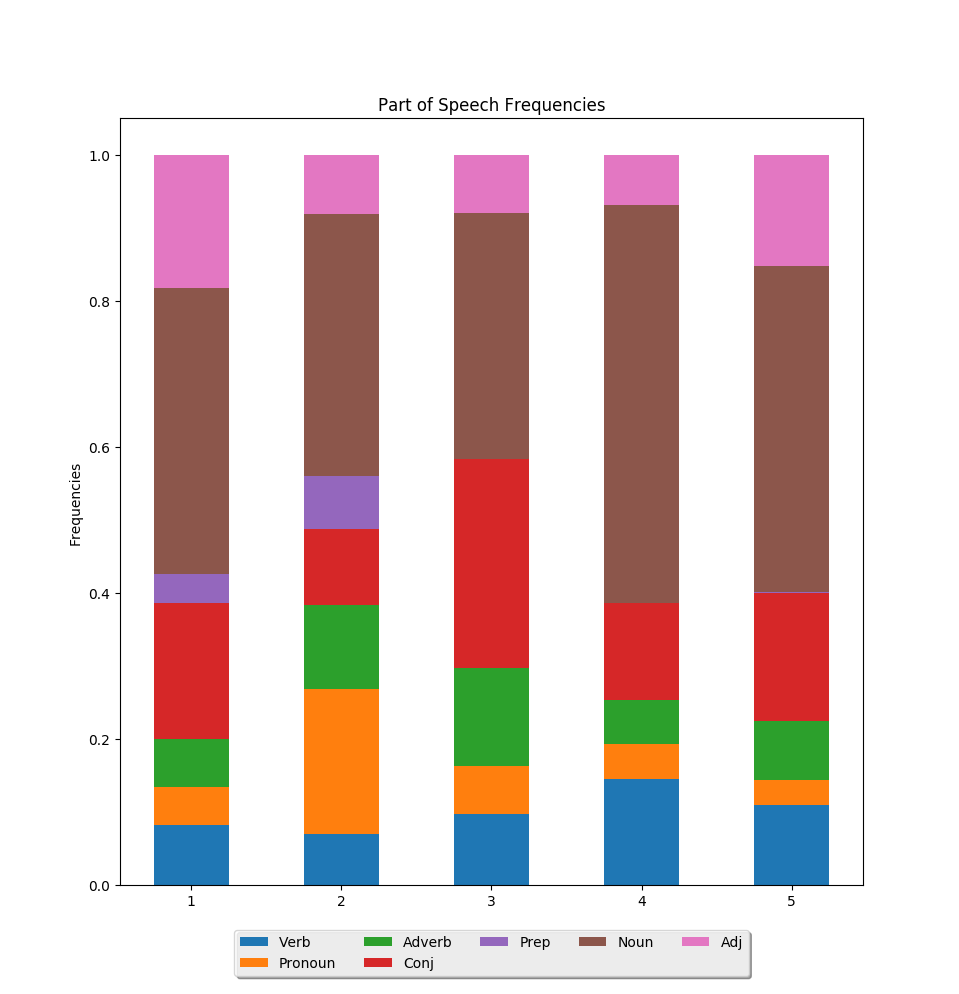
\includegraphics[scale=0.6]{../src/results/parts_of_speech_5}
\end{center}

For the model of 5 hidden states, moderate specialization has occured. In particular, smaller categories such as prepositions and adverbs have significant variance between states. Nouns, however, have similar frequencies across states.

\begin{center}
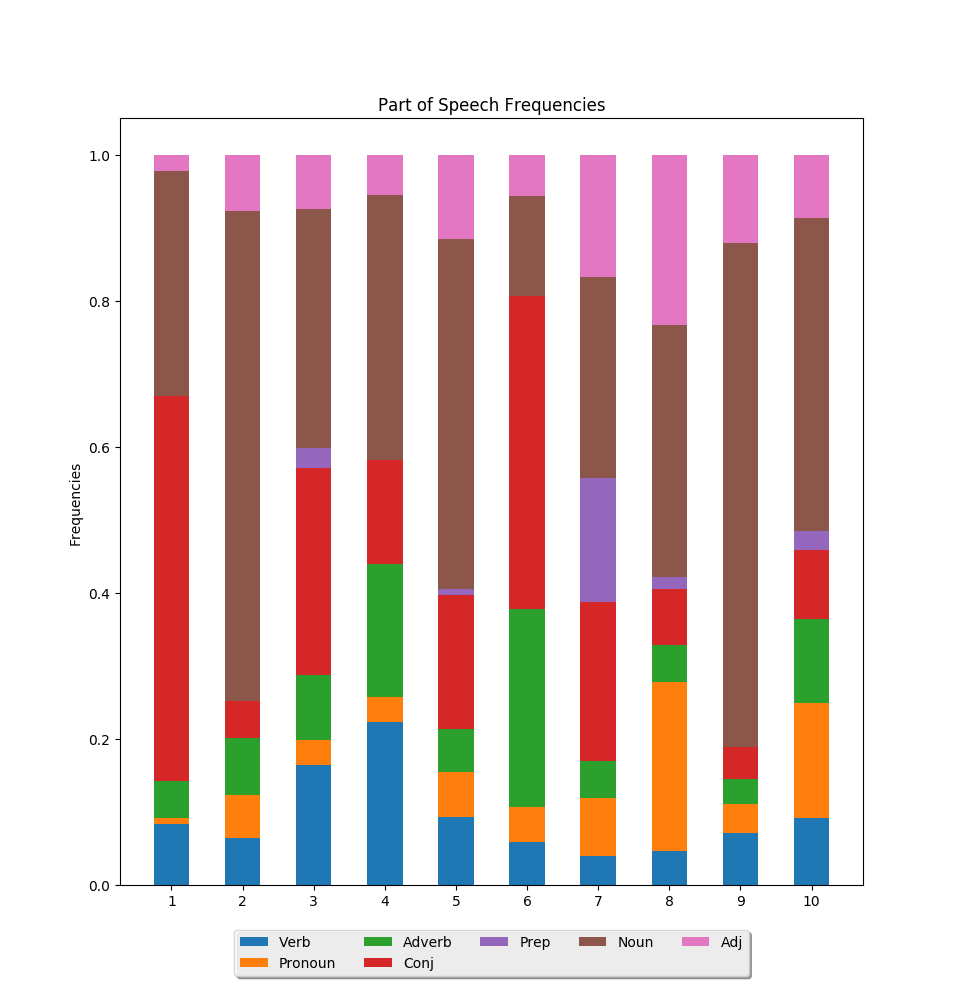
\includegraphics[scale=0.6]{../src/results/parts_of_speech_10}
\end{center}

For the model of 10 hidden states, significant specialization has occured for all parts of speech.

\begin{center}
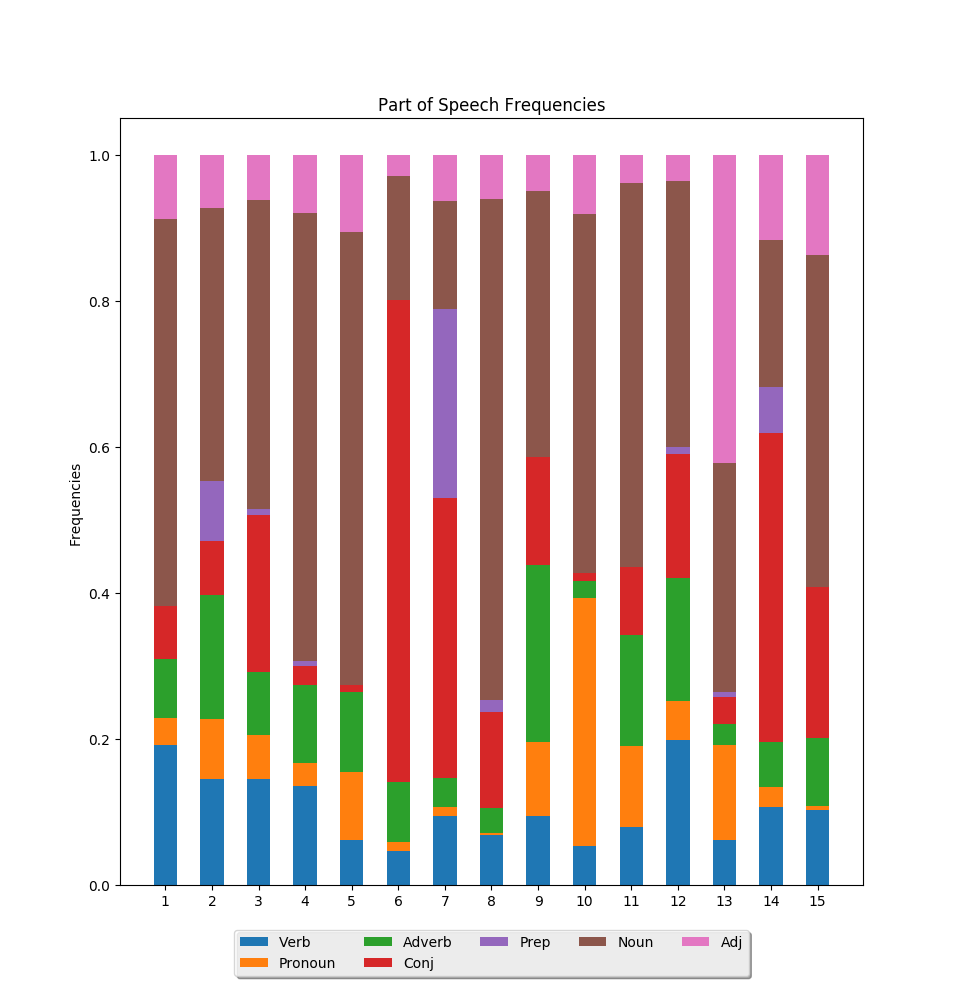
\includegraphics[scale=0.6]{../src/results/parts_of_speech_15}
\end{center}

For the model of 15 hidden states, massive specialization has occured. In particular, prepositions exist almost solely in state 7.

\pagebreak
\section{Appendix C - Syllable Counts}
We trained 3 models, one each of 5, 10, and 15 hidden states. We analyzed how often each state in each model emitted words of different syllabic lengths. We found that, while there were differences between states, they were not as prominent as differences between the frequencies with which states emitted different parts of speech. As a result, it appears more likely that differences in syllable count frequencies are a side effect of the models learning other factors. Note that the data include words with 0 syllables; this is an error on the part of the publicly available code used to count syllables, and in effect represents a reasonable estimate for the error this data. Graphs were generated with Matplotlib.

\begin{center}
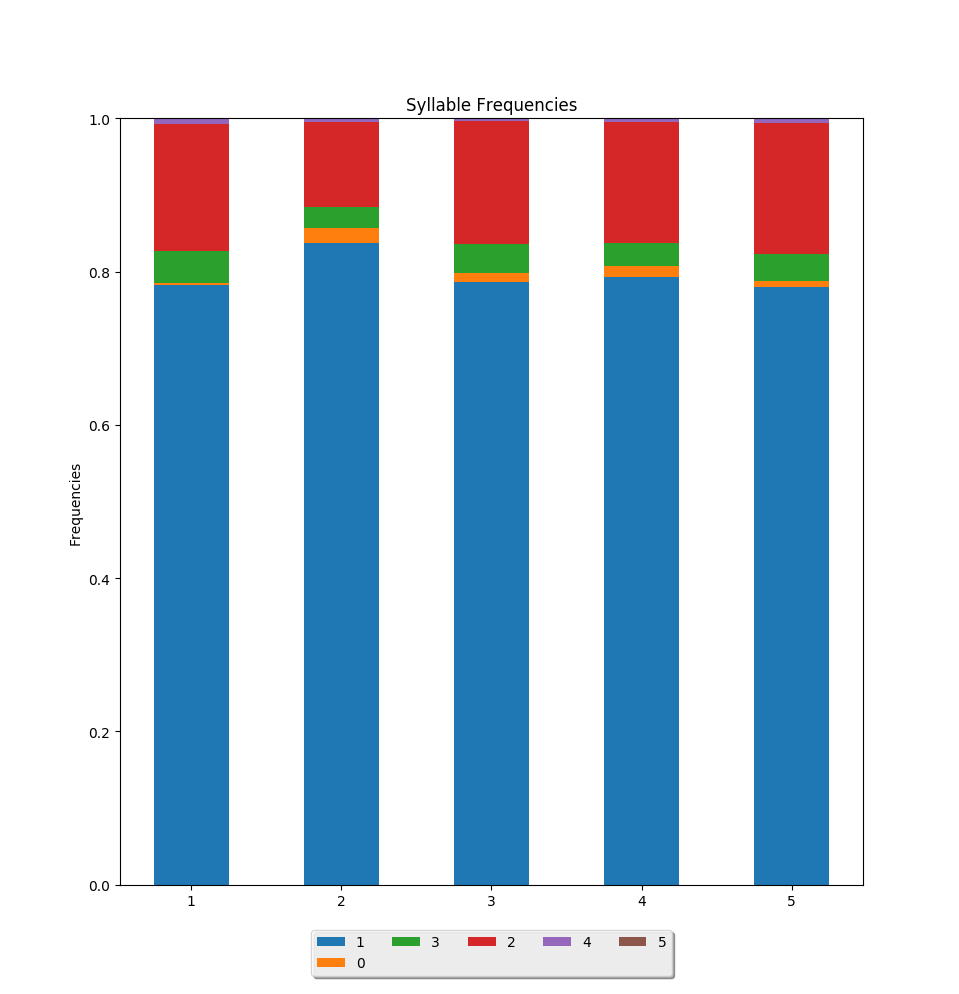
\includegraphics[scale=0.5]{../src/results/syllables_5}
\end{center}

Syllable frequencies for the model of 5 hidden states. Note the lack of variation between states.

\begin{center}
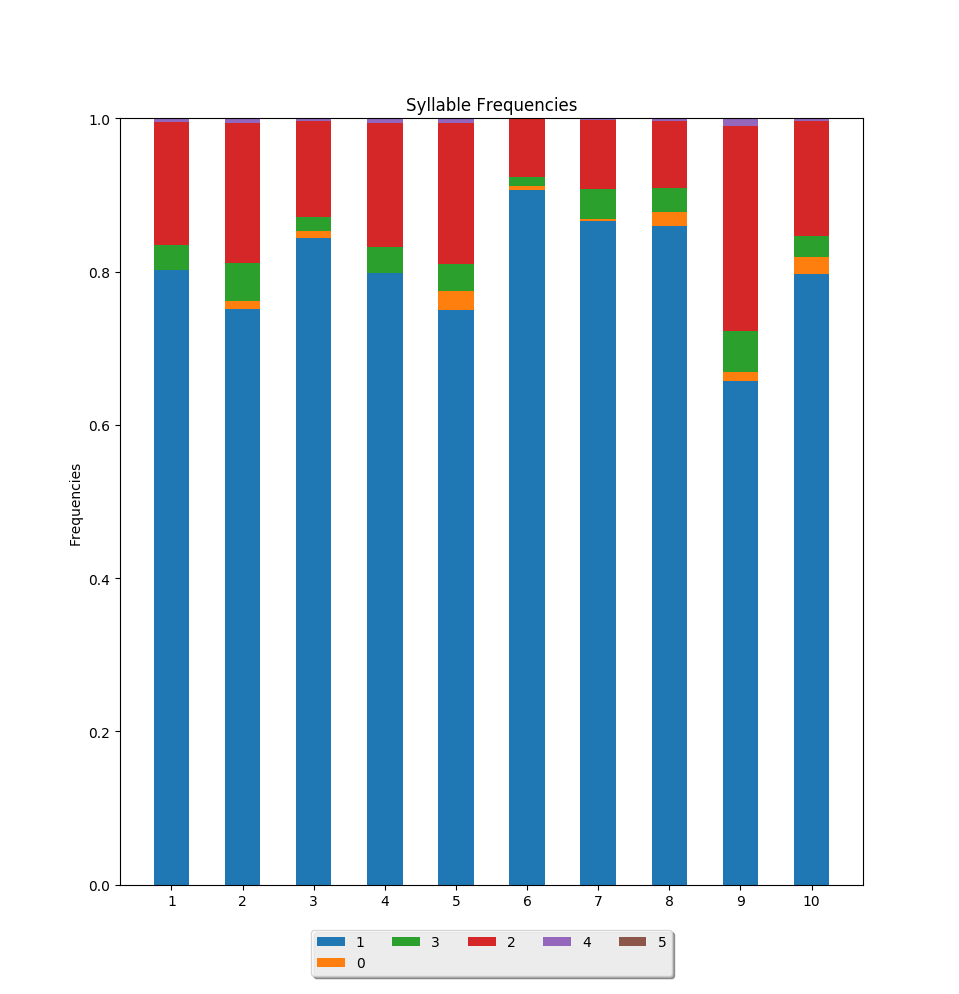
\includegraphics[scale=0.6]{../src/results/syllables_10}
\end{center}

Syllable frequencies for the model of 10 hidden states. This model demonstrates more variance than the model of 5 states, although this is likely an artifact of the model learning other factors (namely, parts of speech).

\begin{center}
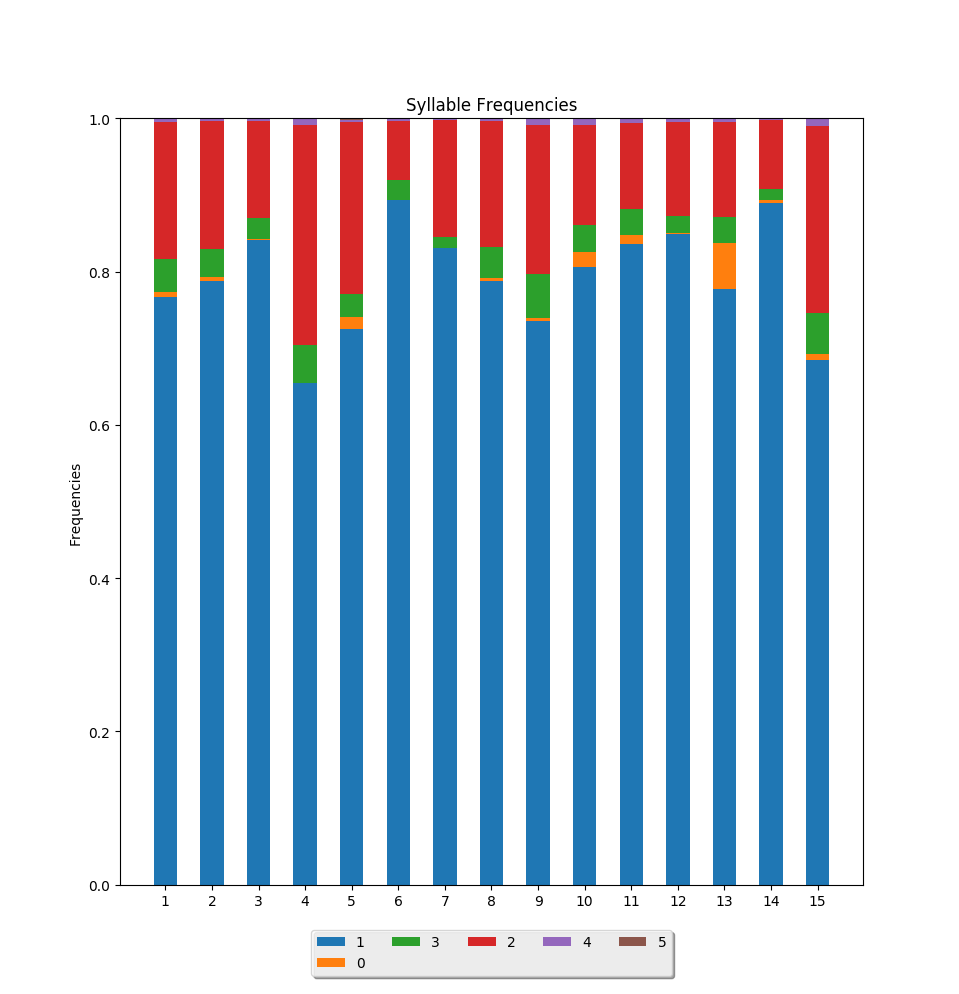
\includegraphics[scale=0.6]{../src/results/syllables_15}
\end{center}

Syllable frequencies for the model of 15 hidden states. As in the model of 10 states, the differences in this data are most likely a side effect of the model learning parts of speech.

\pagebreak
\section{Appendix D - Transition Frequencies}
We visualize the transition frequencies between various states. This information does not explicitly give information about the underlying meaning of states, and is presented here both for completeness and because it is used in visualizing the network of the HMMs.

\begin{center}
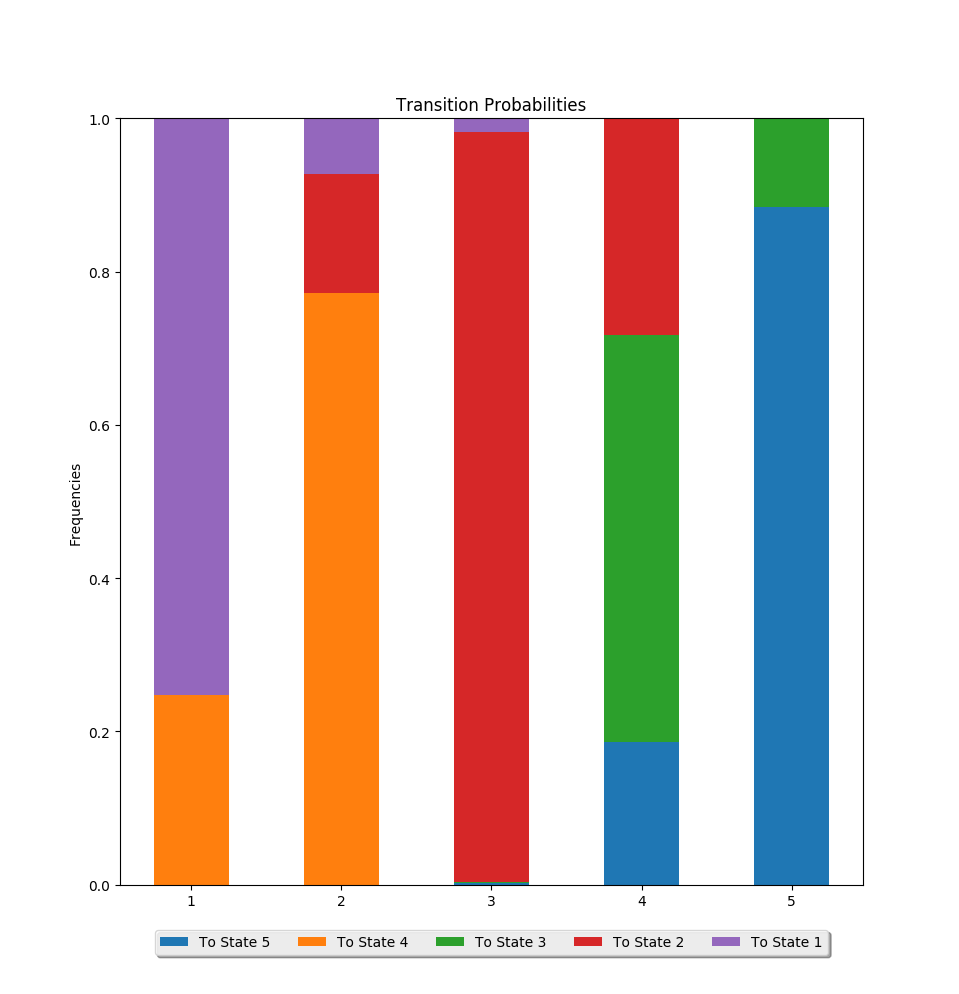
\includegraphics[scale=0.6]{../src/results/transitions_5}
\end{center}

Transition frequencies for the model of 5 hidden states.

\begin{center}
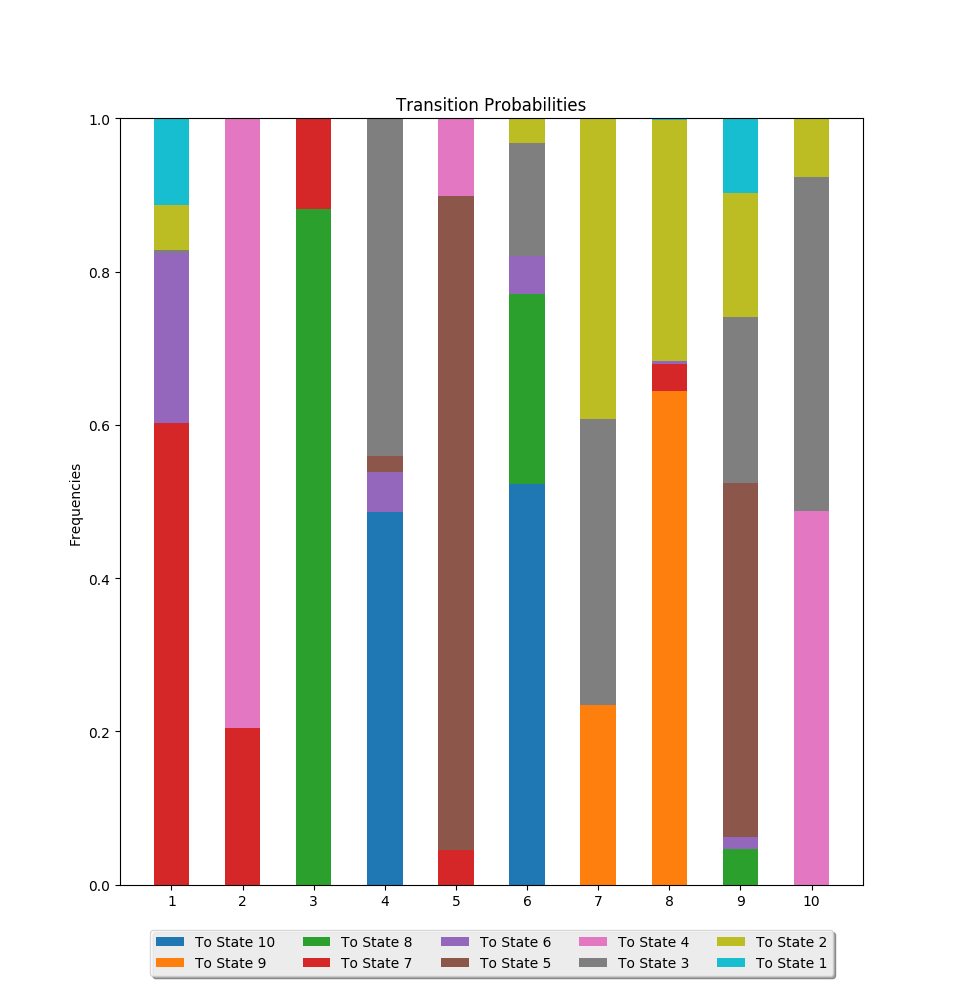
\includegraphics[scale=0.6]{../src/results/transitions_10}
\end{center}

Transition frequencies for the model of 10 hidden states.

\begin{center}
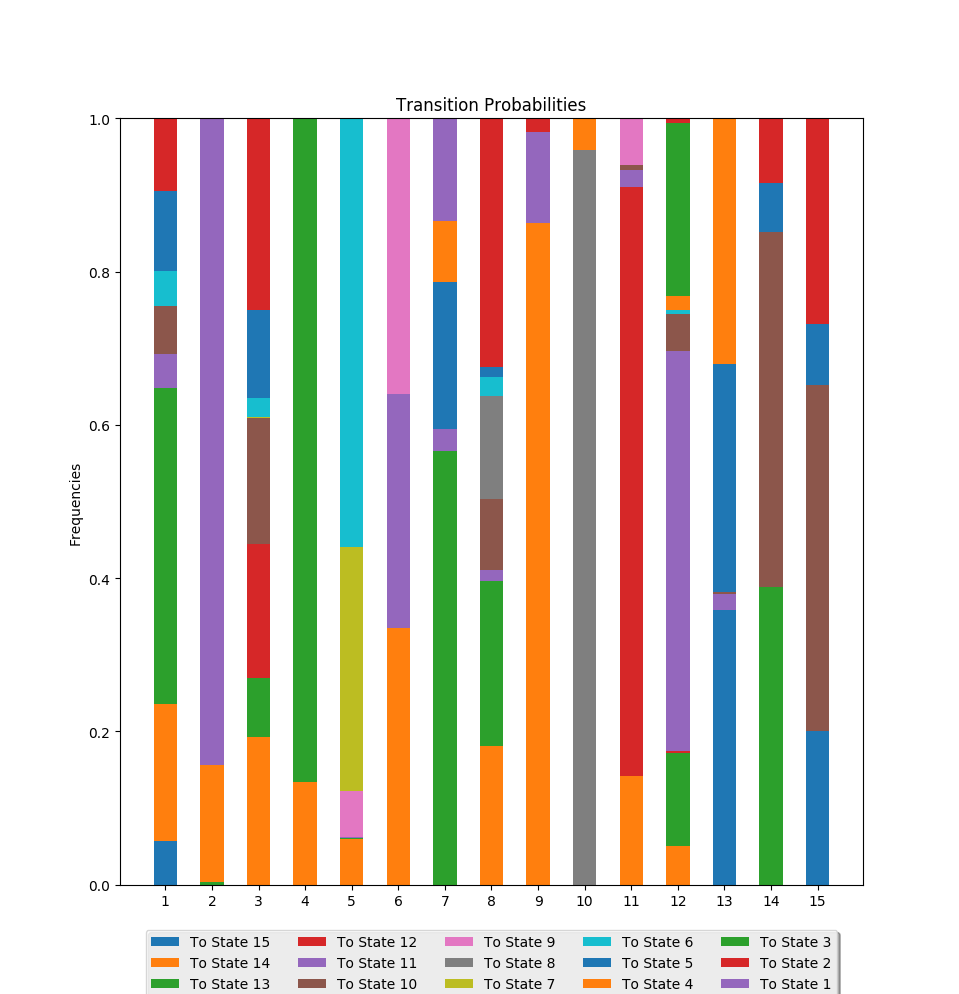
\includegraphics[scale=0.6]{../src/results/transitions_15}
\end{center}

Transition frequencies for the model of 15 hidden states.

\pagebreak
\section{Appendix E - HMM Networks}
We visualize the entire HMM as a network for each model. Each state shows parts of speech that it represents at an unusually high rate (mean + 0.5*std), or (if no part of speech is emitted that frequently) the part of speech that it emits at the highest rate above the mean. Directed edges are added between states when the transition probability is higher than the mean. Given our conclusion that the model learns parts of speech primarily, this provides a visualization of the main parameters learned by our model. Note that the shown parts of speech are those represented disproportionately for the state; this does not mean that the state predominately emits those parts of speech, only that it emits them at an unusually high rate.

\begin{center}
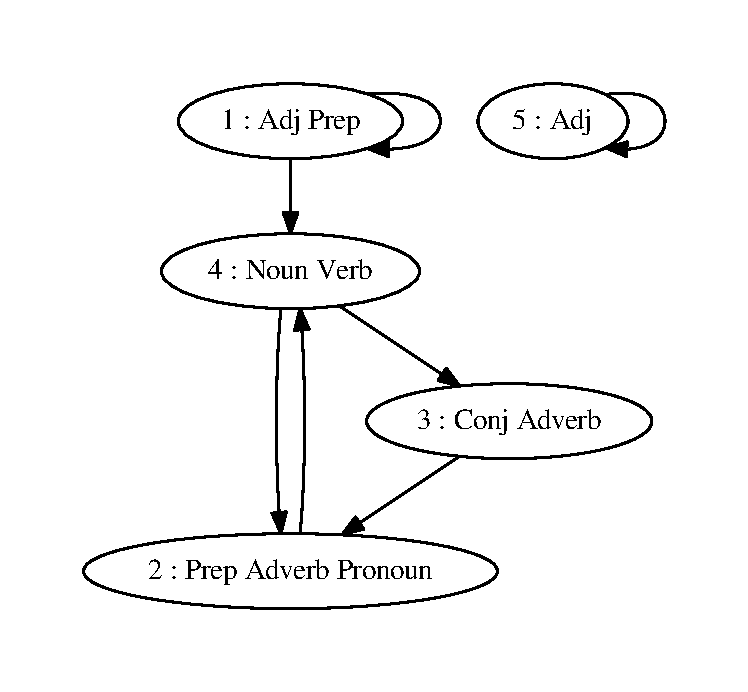
\includegraphics[scale=0.6]{../src/results/graph_5}
\end{center}

Network model for the 5 state HMM. Note the emergence of rudimentary grammatical structure.

\begin{center}
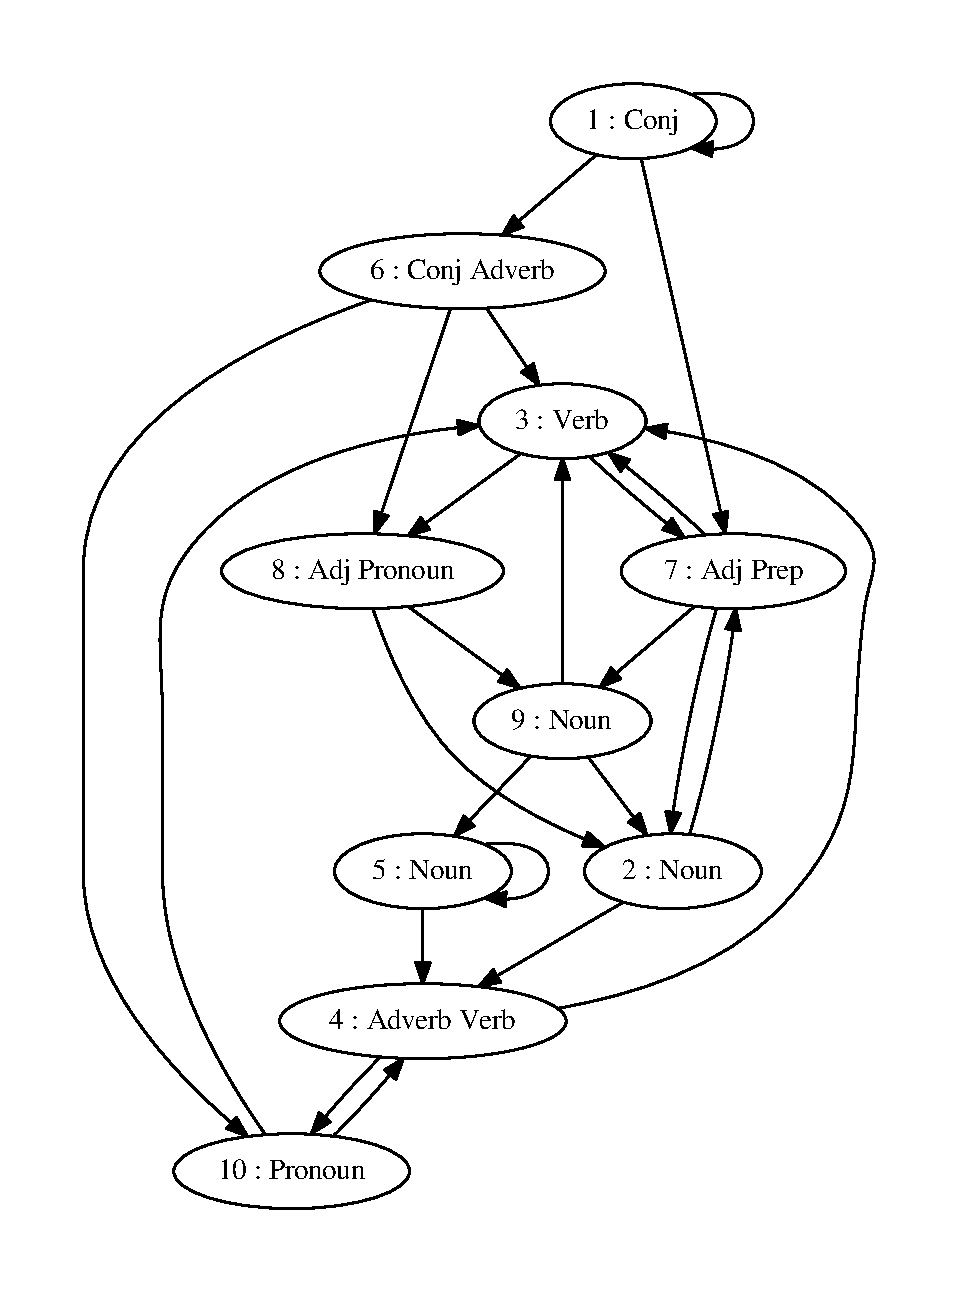
\includegraphics[scale=0.6]{../src/results/graph_10}
\end{center}

Network model for the 10 state HMM. Note the formation of `hubs' at states 2, 3, and 7. Further note the increased grammatical structure evident in the transitions (i.e., Noun states linking to Verb states, Adverbs to Verbs, etc.).

\begin{center}
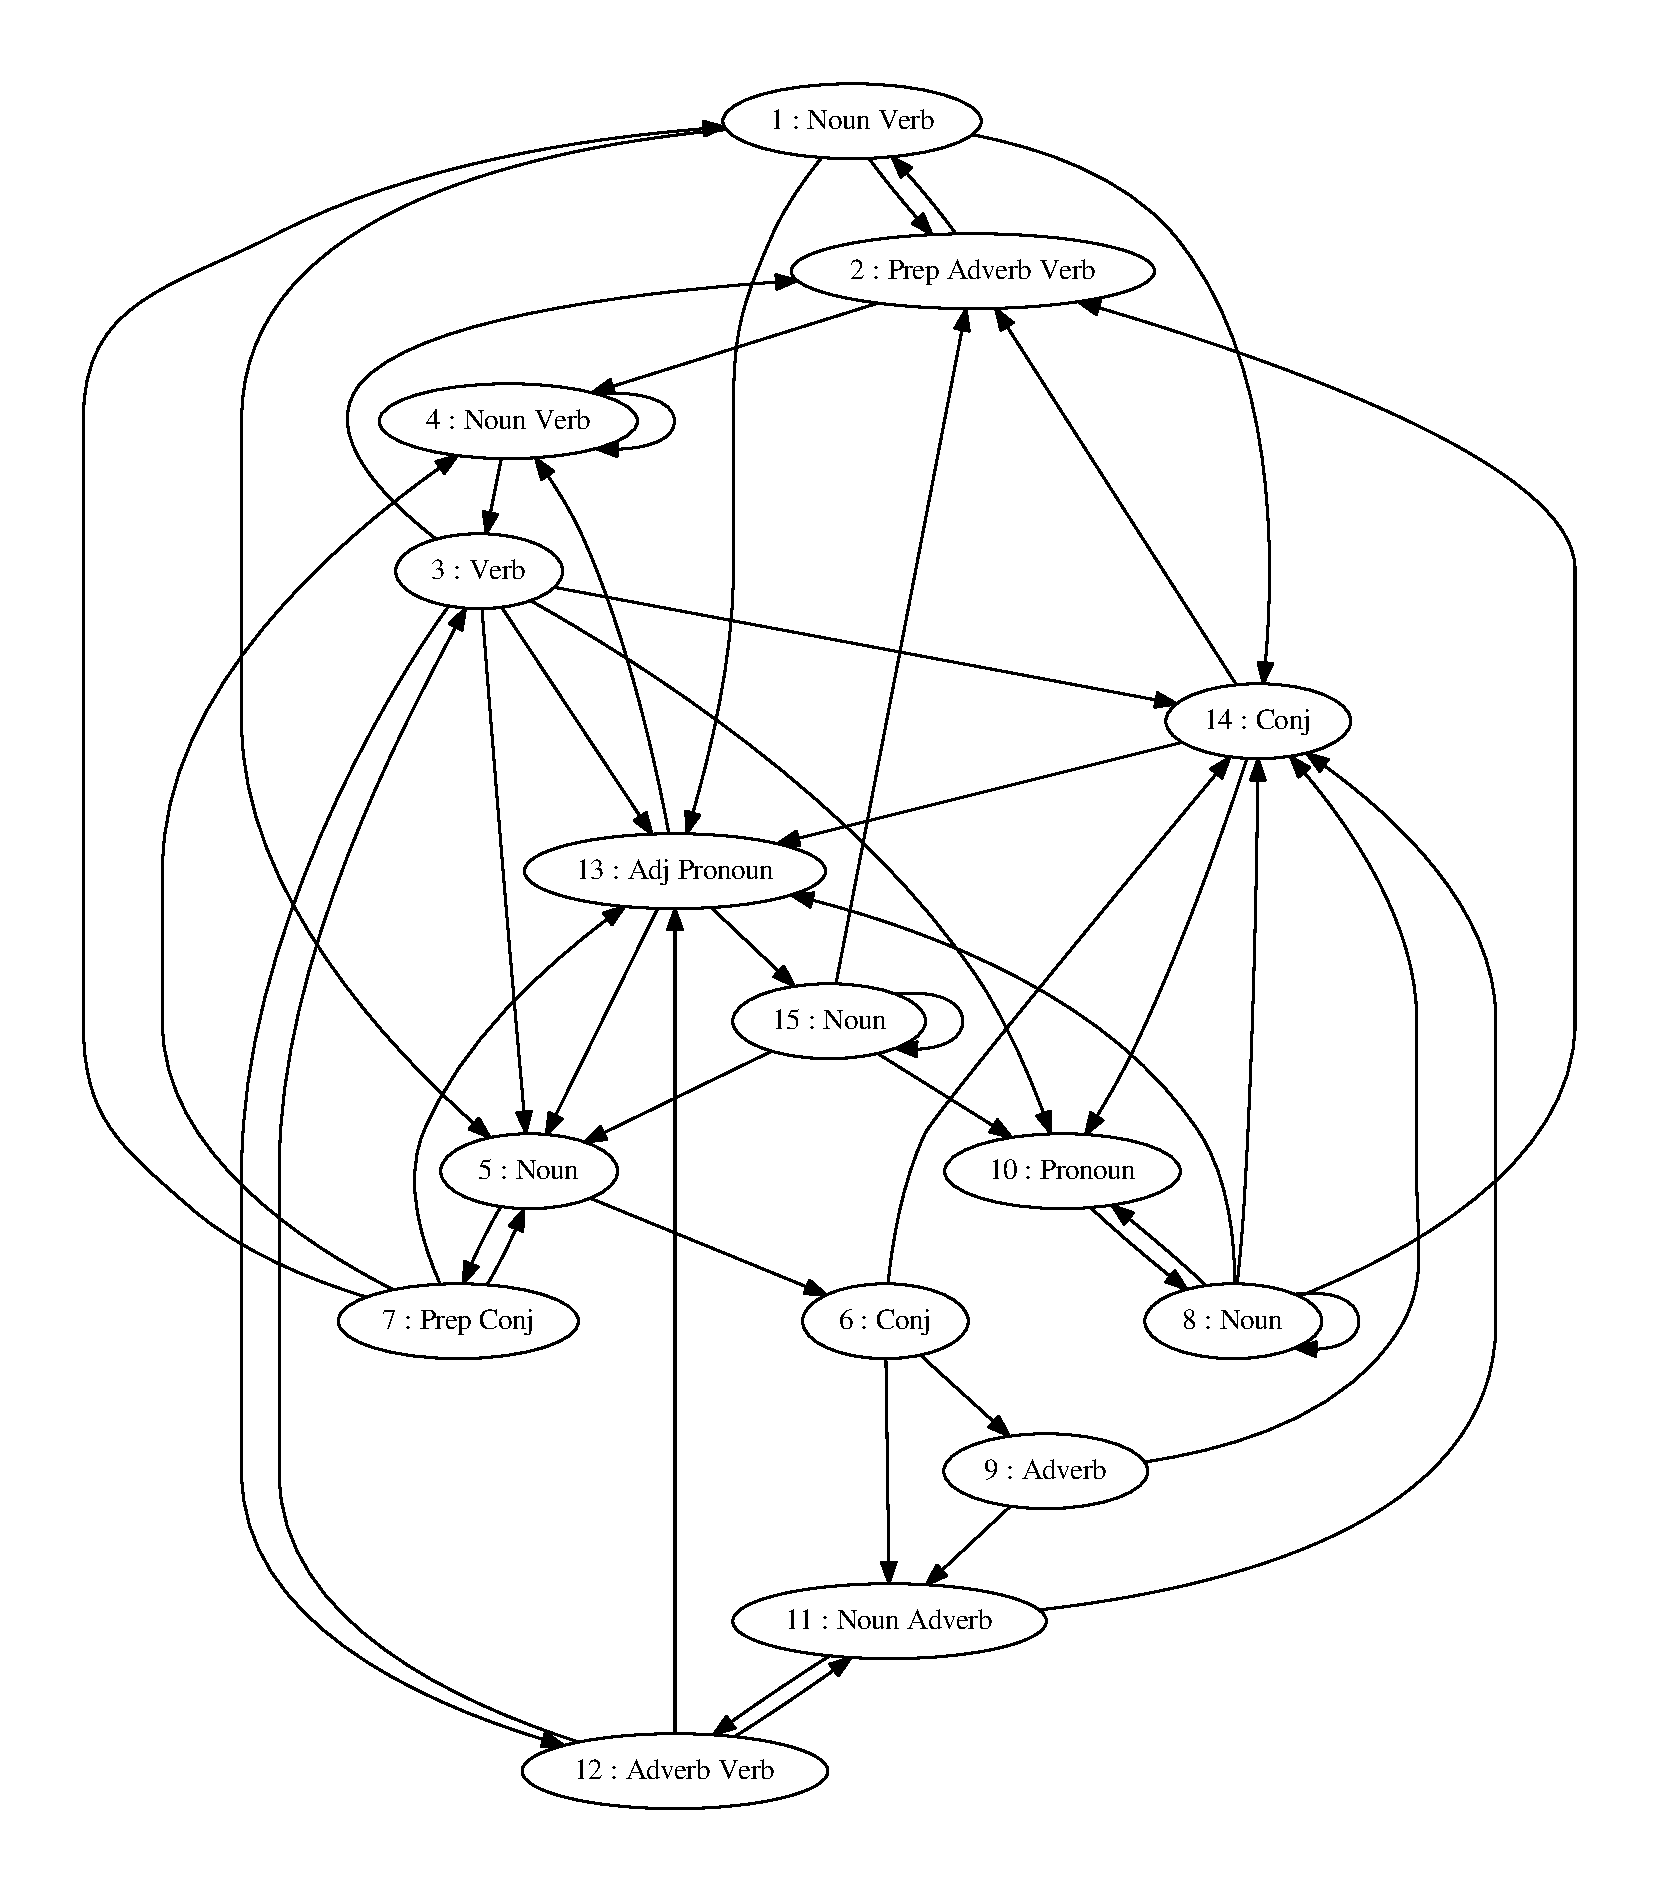
\includegraphics[scale=0.5]{../src/results/graph_15}
\end{center}

Network model for the 15 state HMM. Note the increasing formation of hubs, particularly at states 13 and 14. This is likely a result of the high emission rates of adjectives and conjunctions in 13 and 14, respectively (see Appendix B).

\end{document}